\chapter{Introduction}

\begin{figure}

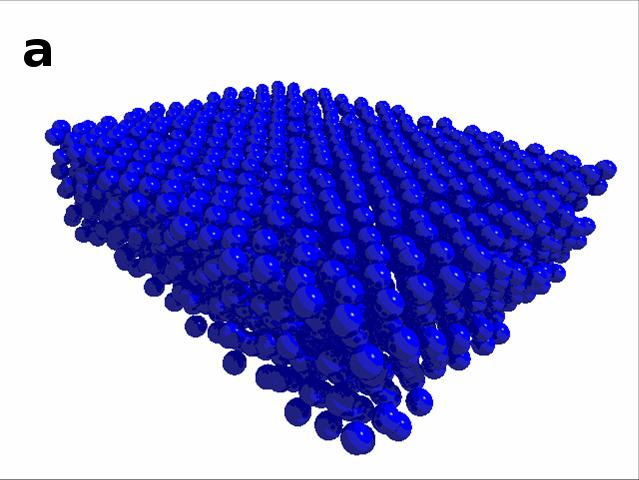
\includegraphics[width=0.45\linewidth]{figures/literature-review/sphere-crystal.png}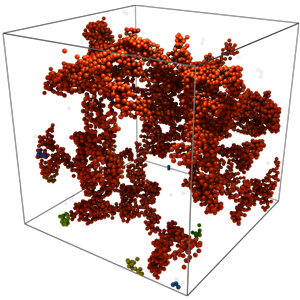
\includegraphics[width=0.45\linewidth]{figures/literature-review/sphere-gel.png}
\caption{Spherical colloids with purely repulsive interactions may assemble into (a) ordered 
crystal structures with fcc geometry or (b) space-filling disordered ``glass'' structures. Attractive
colloids assemble into (c) open ``gel'' structures.}

\label{fig:isotropic-structs}

\end{figure}

As a class of materials, self-assembled colloidal structures are of interest in applications as widely varied
as photonic crystals~\ref{?}, photovoltaic devices~\ref{?}, and three-dimensional templates for tissue 
engineering scaffolds~\ref{?}. However, despite the wide interest in these structures, the range of possible 
structures made available by self-assembled spherical colloids is relatively narrow.  Due to the isotropic nature
of colloidal interactions, there are three basic structures available.~\ref{?}  When the interparticle interaction is purely 
repulsive, such as in a hard-core interaction, two structures are available: a stable, ordered face-centered-cubic crystal
structure(Fig.~\ref{fig:isotropic-structs}(a)) with a volume fraction of ??, and a dynamically-trapped disordered ``glassy''
state (Fig.~\ref{fig:isotropic-structs}(b)) with a slightly higher volume fraction of up to ??.  Both of these 
structures are space-filling in the sense that there are no large gaps in the structure larger than the 
particle size.  When the interparticle interaction is attractive, the particles may form an open, disordered ``gel'' 
structure (Fig~\ref{fig:isotropic-structs}(c)) 
with an essentially random arrangement and gap volumes which are potentially larger than the particle size~\ref{?}.

Many applications, such photonic crystals, would benefit from the availability of ordered structures with different geometries
than fcc.  One potential route for realizing different structures is to change the building block, replacing the 
isotropically-interacting spherical particles with some type of anisotropic particle.  Here, we develop techniques for
the fabrication of colliods with geometric and chemical anisotropy and begin to characterize the dynamical behavior
and self-assembly of these particles.

\section{Thesis Scope}

The aim of this work is to develop techniques for the fabrication and characterization of anisotropic colloids, and begin
to explore their dynamical and assembly characteristics.  Fabrication is based on flow lithography
techniques for producing polymeric particles~\ref{doyle-cfl, doyle-sfl}, 
and characterization is primarily based on fluorescence and confocal microscopy.
The systems used are based on a combination of a hydrophobic monomer (tri(methylol propane) triacrylate) and hydrophilic 
monomers (poly(ethylene glycol) diacrylate and 20-mol ethoxylated tri(methylol propane) triacrylate). 
Single-component particles are used to study the effects of
geometry on dynamical behavior in isolation, while multiple-component particles introduce 
the hydrophobic attraction for self-assembly.  The solvents used are 
varied to explore this interaction, and include
water, ethanol, dimethyl sulfoxide, isopropanol and toluene.

\section{Thesis Organization}

A review of the relevant literature on the fabrication of anisotropic colloids, their experimental and simulated
self-assembly, and their characterization using particle tracking techniques is included in chapter two.  Chapter three
details algorithms and software developed in the course of this study to analyze microscopy images containing 
anisotropic colloids.  Chapter four investigates the fabrication, behavior and self-assembly of simple rod-shaped colloids
in both single-component and ``Janus'' forms, while chapter five investigates colloids with more exotic geometries. The main
conclusions are presented in chapter six.  Appendices are included which present experimental techniques developed for but not used
in the final study, including novel microfluidic devices for studying concentrated colloids and a variant of the fabrication
technique.
